\lecture
Faserweise kann man nun Konstruktionen der linearen Algebra vornehmen: direkte Summe, Tensorprodukt, Dualraum etc.

\begin{exmp}
	\begin{enumerate}[label={\roman*})]
		\item Direkte Summe:\\
			Seien $ (E,\pi,B),(\tilde{E},\tilde{\pi},\tilde{B}) $ Vektorbündel über $B$. Dann ist die \emph{direkte Summe}
			\[ E \oplus \tilde{E} := \bigcup_{x \in B} E_x \oplus \tilde{E}_x \]
			auch wieder ein Vektorbündel (von Rang $n + \tilde{n}$)
		\item Tensorprodukt:
			\[ E \otimes \tilde{E} := \bigcup_{x \in B} E_x \otimes \tilde{E}_x \]
		Bündel-Atlas:
			\begin{gather*}
				\left\{ (\varphi \otimes \psi, U \cap V) \mid (\varphi,U) \in \ \text{Atlas von }E, (\psi,V) \in \ \text{Atlas von } \tilde{E} \right\}\\
				\bound{\varphi \otimes \psi}{E_x \otimes \tilde{E}_x} : E_x \times \tilde{E}_x \to \{x\} \times \R^n \otimes \R^{\tilde{n}}
			\end{gather*}
		\item Duales Bündel: $ E^* = \bigcup_{x \in B} E_x^* $\\
			$ \pi_{E^*} $ so, dass $ \pi_{E^*}^{-1} (x) = E_x^* = \Hom{E_x,\R} $\\
			Bündelatlas: Ist $ (\psi,U) \in $ Atlas von $E$, so ist $ \begin{aligned}[t]
				\psi^*: \pi_{E^*}^{-1} (U) &\to U \times \R^n\\
				E_x^* \ni \alpha_x &\mapsto (x,w)
			\end{aligned} $, wobei $w$ der eindeutige Vektor $\in \R^n$ ist, sodass
			\[ \alpha_x (v_x) = \langle w,pr_2(\underbrace{\psi(v_x)}_{\in \{x\} \times \R^n}) \rangle \quad \foralll v_x  \in E_x \]
	\end{enumerate}
\end{exmp}

Speziell für das Tangentialbündel:

\begin{defn}[Kotangentialbündel]\index{Vektorraumbündel!Kotangentialbündel}
	Das \emph{Kotangentialbündel} $T^*M$ an einer differenzierbaren Mannigfaltigkeit $M$ ist das zu $TM$ duale Bündel. $ (T_pM)^* =: T_p^*M $ heißt \emph{Kotangentialraum}.
\end{defn}

In Koordinaten: Seien $ (x_1,\dotsc,x_n) $ lokale Koordinaten bei $p \in M$, $ \left( \bound{\del_{x_1}}{p},\dotsc, \bound{\del_{x_n}}{p} \right) $ eine Basis von $T_pM$. Hierbei betrachten wir nicht unbedingt bei $p$ zentrierte Karten $ (\varphi,U) $ von $M$.\\
Es ist dann für $f \in C^\infty(U)$ beziehungsweise Keim bei $p$
\begin{align*}
	\bound{\del_{x_j}}{p}f &= \bound{\del_{x_j}}{\varphi(p)} (f \circ \varphi^{-1})\\
	&= \del_{x_j} \hat{f} (\hat{p}),
\end{align*}
mit $\hat{p} = \varphi(p)$ und $\hat{f} = f \circ \varphi^{-1}$ als Koordinatendarstellung von $f$.

\begin{rem}
	Kartenwechsel
	\image{3_20}{8cm}
	Die Tangentialabbildung $T_p\Phi$ bezüglich der Basen $ (\del_{x_1},\dotsc, \del_{x_n}),(\del_{y_1},\dotsc,\del_{y_n}) $ ist die Jacobimatrix $ \begin{pmatrix}
		\del_{x_1} \Phi_1 & \cdots & \del_{x_n}\Phi_1\\
		\vdots & &\vdots\\
		\del_{x_1}\Phi_n & \cdots & \del_{x_n}\Phi_n
	\end{pmatrix} = D\Phi, $ also $ T_p\Phi(\del_{x_i}) = \sum \del_{x_i}\Phi_j ({\vertarrowbox[3pt]{\hat{p}}{Koord. von $p$, also $\varphi(p)$}}) \del_{y_j}. $
\end{rem}

Merke: $ \Phi_j(\hat{p}) = \psi_j(p) = y_j $\\
Man schreibt daher auch
\[ \bound{\del_{x_i}}{p} = \sum_{j=1}^{n} \frac{\del y_j}{\del x_i}(p) \bound{\del_{y_j}}{p} \]
Denn $T_p\Phi$ transponiert nicht in einen anderen Tangentialraum, sondern bildet wieder (sogar isomorph) nach $T_pM$ ab. (Basiswechsel!)\\
In der Notation unterscheiden wir $p$ und $\hat{p}$, $f$ und $\hat{f}$ meist nicht.

\begin{exmp}
	\begin{enumerate}[label={\roman*})]
		\item $ M = \R^2 $, kartesische vs. Polarkoordinaten\\
			$ \Phi = \psi \circ \varphi^{-1}, \varphi^{-1}(r,\theta) = \begin{pmatrix}
				r \cos \theta \\ r \sin \theta
			\end{pmatrix}, r \in \R_{\geq 0}, \theta \in (0,2\pi), \psi(x_1,x_2) = \begin{pmatrix}
			x_1\\x_2
			\end{pmatrix} $\\
			Betrachte $v \in T_p\R^2, v = \bound{\del_r}{p} - \bound{\del_\theta}{p},\ p = \begin{pmatrix}
				0\\2
			\end{pmatrix},\ (r=2,\theta = \frac{\pi}{2})$\\
			\begin{minipage}{\linewidth}
				\begin{wrapfigure}{R}{4cm}
					\centering
					\includegraphics[width=4cm]{3_21 i}
				\end{wrapfigure}
				
				$ \del_r \Phi \left(2,\frac{\pi}{2} \right) = \begin{pmatrix}
					0\\1
				\end{pmatrix}, \quad \del_\theta \Phi \left( 2,\frac{\pi}{2} \right) = \begin{pmatrix}
					-2\\0
				\end{pmatrix} $\\
				$ \implies \begin{aligned}[t]
					\bound{\del_r}{p} &= 0 \cdot \bound{\del_{x_1}}{p} + \bound{\del_{x_2}}{p}\\
					\bound{\del_\theta}{p} &= -2 \bound{\del_{x_1}}{p}
				\end{aligned} $\\
				$ \implies v $ hat in kartesischen Koordinaten die Darstellung $ \bound{\del_{x_2}}{p} + 2 \bound{\del_{x_1}}{p} $
			\end{minipage}
		\item $ \Phi(x,y) = \begin{pmatrix}
			x\\p+x^3
			\end{pmatrix} = \begin{pmatrix}
				\tilde{x}\\\tilde{y}
			\end{pmatrix}, p = \begin{pmatrix}
				1\\0
			\end{pmatrix} $\\
			$ \bound{\del_x}{p}\Phi = \begin{pmatrix}
				1\\3
			\end{pmatrix}, \bound{\del_y}{p}\Phi = \begin{pmatrix}
				0\\1
			\end{pmatrix} $\\
			$ \implies \begin{aligned}[t]
				\bound{\del_x}{p} &= \bound{\del_{\tilde{x}}}{p} + 3\bound{\del_{\tilde{y}}}{p} \neq \bound{\del_{\tilde{x}}}{p} \ \text{obwohl } \tilde{x} = x\ \text{ist}\\
				\bound{\del_y}{p} &= \bound{\del_{\tilde{y}}}{p}
			\end{aligned}$
	\end{enumerate}
\end{exmp}

\begin{rem}\label{3.22}
	Beachte: Schreibt man ein Element $v \in T_pM$ als $ v = \sum v_i \bound{\del_{x_i}}{p} = \sum \tilde{v}_j \bound{\del_{y_j}}{p} $, so gilt also
	\[ \sum_{i=1}^{n} v_i \bound{\del_{x_i}}{p} = \sum_{i=1}^{n} v_i \sum_{j=1}^n \frac{\del\Phi_j}{\del x_i}(\hat{p}) \bound{\del_{y_j}}{p}, \]
	\[ \text{Also } \tilde{v}_j = \sum_{i=1}^n \del_{x_i} \Phi_j(\hat{p}) v_i\quad \text{"kovariantes Transformationsverhalten"} \]
	Wie transformieren sich Elemente des Kotangentialraums? Sei $w \in T_pM^*$. Bezeichne $ (\bound{\alpha_1}{p},\dotsc, \bound{\alpha_n}{p}) $ die zu $ (\del_{x_1},\dotsc, \del_{x_n}) $ duale Basis, $ (\bound{\tilde{\alpha}_1}{p},\dotsc, \bound{\tilde{\alpha}_n}{p}) $ die zu $ (\del_{y_1},\dotsc, \del_{y_n}) $. Dann schreibt sich $w$ als 
	\[ w = \sum w_i \bound{\alpha_i}{p} = \sum \tilde{w}_j \bound{\tilde{\alpha}_j}{p}, \]
	wobei $w_i = w \left( \bound{\del_{x_i}}{p} \right)$ und $\tilde{w}_j = w \left( \bound{\del_{y_j}}{p} \right)$. Somit folgt
	\begin{align*}
		w_i &= w \left( \bound{\del_{x_i}}{p} \right) = w \left( \sum_{j=1}^n \underbrace{\del_{x_i} \Phi_j(\hat{p})}_{\in \R} \bound{\del_{y_j}}{p} \right)\\
		&= \sum_{j=1}^n \del_{x_i} \Phi_j(\hat{p}) \tilde{w}_j\quad \text{"kontravariantes Transformationsverhalten"}
	\end{align*}
	Beziehungsweise für die Basis:
	\[ \tilde{\alpha}_j = \sum_{i=1}^n \del_{x_i}\Phi_j (\hat{p}) \bound{\alpha_i}{p} \]
\end{rem}

\begin{defn}[Differential-Eins-Form]\index{Vektorraumbündel!Differential-Eins-Form}
	Ein glatter Schnitt $T^*M \to M$ heißt \emph{Differential-Eins-Form}. Die Menge der Differentialformen bezeichnet man mit $\Omega^1(M)$. Ist $U \subset M$ offen, so bezeichnet man die Menge der glatten Schnitte $ \bound{T^*M}{U} \to U $ mit $\Omega^1(U)$.
\end{defn}

In Koordinaten: Die Koeffizientenfunktion hängt glatt von $p \in M$ ab:

\begin{exmp*}
	$p \mapsto T_pf,\ f \in C^\infty(M)$, das Differential von $f$ ist $\in \Omega^1(M)$. Man schreibt dafür auch $df$ (anstelle von $p \mapsto T_pf$). Denn:\\
	In Koordinaten gilt $ T_pf \left( \bound{\del_{x_i}}{p} \right) = \del_{x_i} f(p) $ (denn $T_pf$ ist in dieser Basis die Jacobimatrix!), das heißt $\bound{df}{p}$ lässt sich schreiben als
	\[ \bound{df}{p} = \sum_{i=1}^n \del_{x_i} f(p) \bound{\alpha_i}{p} \quad \leftarrow \text{duale Basis zu }\del_{x_1},\dotsc, \del_{x_n} \]
	Insbesondere gilt für die Koordinatenfunktion $ f = x_j: \bound{dx_j}{p} = \bound{\alpha_j}{p}. $\\
	Diese Notation wollen wir daher im Folgenden für die duale Basis verwenden.
\end{exmp*}

\begin{lem}
	Sei $ (\varphi,U) $ eine Karte von $M$ bei $p \in U$. Dann lässt sich jedes $ \alpha \in \Omega^1(M) $ schreiben als
	\[ \alpha = \sum_{i=1}^n f_i d x_i, \]
	$dx_i \in \Omega^1(U)$, mit $f_i \in C^\infty(U)$ eindeutig bestimmt.
\end{lem}

\begin{exmp*}
	$ \Phi(r,\theta) = \begin{pmatrix}
		r\cos\theta\\ r \sin\theta
	\end{pmatrix} $\\
	$\alpha \in \Omega^1(\R^2) \implies w = f(x,y)dx + g(x,y)dy$, $f$ und $g$ glatt.\\
	Wir könnten die Formel aus \ref{3.22} verwenden,
	\[ \bound{\tilde{\alpha}}{p} = \sum_{i=1}^n \del_{x_i} \Phi_j (\hat{p}) \bound{\alpha_i}{p}, \]
	schneller geht es direkt:
	\begin{align*}
		dh &= \sum \del_{y_j}h dy_i\\
		d(r\cos\varphi) &= \cos\varphi dr - r \sin\varphi d\varphi\\
		d(r\sin\varphi) &= \sin\varphi dr + r \cos\varphi d\varphi
	\end{align*}
	\begin{align*}
		\implies w &= \Big(f \big(r\cos\theta,r\sin\theta \big)\cos\theta + g \big(r\cos\theta,r\sin\theta \big)\sin\theta\Big) dr\\
		&+ r\Big(-f \big(r\cos\theta,r\sin\theta \big)\sin\theta + g \big(r\cos\theta,r\sin\theta \big)\cos\theta\Big) d\theta
	\end{align*} 
\end{exmp*}